\documentclass[aspectratio=169]{beamer}
\usepackage{simplemetropolis} % Load your custom style
% % Input encoding.
\usepackage[utf8]{inputenc} % For accents in spanish: transforms "á" into "\'a"
\usepackage[T1]{fontenc} % Output encoding. Use to avoid silly problems on the output.
                         % See: http://tex.stackexchange.com/questions/664/why-should-i-use-usepackaget1fontenc
\usepackage{lmodern} % Latin Modern fonts have broader support
% AMS packages
\usepackage{amsmath}
\usepackage{amsfonts}
\usepackage{amssymb}
\usepackage{amsthm}
\usepackage{bbm}
% Other maths packages
\usepackage{mathtools}
\usepackage{leftindex}
% Tables
\usepackage{booktabs}  % For professional tables
\usepackage{multirow}  % For multirow formatting
% Include animated gifs
\usepackage{animate}
% Hyperlink
\usepackage{hyperref}
\hypersetup{
	final,
    bookmarksnumbered=true,
    bookmarksopen=true,
    bookmarksopenlevel=0,
    unicode=false,          % non-Latin characters in Acrobat?s bookmarks
    pdftoolbar=true,        % show Acrobat?s toolbar?
    pdfmenubar=true,        % show Acrobat?s menu?
    pdffitwindow=false,     % window fit to page when opened
    pdftitle={Quantitative Methods For Humanities},    % title
    pdfdisplaydoctitle=true, %display document title instead of file name in title bar
    pdftoolbar=true,
    pdfmenubar=true,
    pdflang={English},
    pdfauthor={Abel Guada Azze},     % author
    pdfsubject={Quantitative Methods For Humanities},   % subject of the document
    pdfcreator={Abel Guada Azze},   % creator of the document
    pdfproducer={Abel Guada Azze}, % producer of the document
    pdfkeywords={Quantitative Methods} {R}, % list of keywords
    pdfnewwindow=true,      % links in new window
    breaklinks=true,
    hidelinks,
    colorlinks,
    linkcolor=CUNEFOrange,          % color of internal links (change box color with linkbordercolor)
    citecolor=black,        % color of links to bibliography
    filecolor=cyan,      % color of file links
    urlcolor=magenta           % color of external links
}
% Import icons
\usepackage{fontawesome}
\usepackage{tikz}
% \pgfplotsset{compat=1.18}
% \usepackage{tkz-euclide}
\usetikzlibrary{shapes,arrows,matrix,positioning,calc}
\newcommand{\tikzmark}[1]{\tikz[baseline,remember picture] \coordinate (#1) {};}
% Define colors
\definecolor{amber}{rgb}{1.0, 0.49, 0.0} % Normalized RGB
\definecolor{firebrick3}{RGB}{207, 33, 32} % 8-bit RGB
\definecolor{deepskyblue3}{RGB}{0, 155, 206} % 8-bit RGB
\definecolor{darkorange3}{RGB}{206, 102, 0} % 8-bit RGB
\definecolor{darkolivegreen3}{RGB}{163, 207, 91} % 8-bit RGB
\definecolor{purpleR}{RGB}{160, 32, 240}
% Customizable new commands
\usepackage{xparse}
% Plain macros
\newcommand{\R}{\mathbb{R}} % real number set
\newcommand{\N}{\mathbb{N}} % natural number set
\newcommand{\lp}{\left(} % left parenthesis
\newcommand{\rp}{\right)} % right parenthesis
\newcommand{\lb}{\left[} % left brackets
\newcommand{\rb}{\right]} % right brackets
\newcommand{\lc}{\left\{} % left curly brackets
\newcommand{\rc}{\right\}} % right curly brackets
\newcommand{\la}{\langle} % left angled brackets
\newcommand{\ra}{\rangle} % right angled brackets
\newcommand*{\defeq}{\mathrel{\vcenter{
                     \baselineskip0.5ex\lineskiplimit0pt
                     \hbox{\scriptsize.}\hbox{\scriptsize.}
                     }}%
                     =}
                     \newcommand{\Rcoef}{\textsf{R}^2} % Coefficient of determination
\newcommand{\adjRcoef}{\oline{\textsf{R}}^2} % Coefficient of determination
\newcommand{\SER}{\textsf{SER}} % Standard error of the regression
\newcommand{\SSR}{\textsf{SSR}} % Sum of squared residuals
\newcommand{\ESS}{\textsf{ESS}} % explained sum of squares
\newcommand{\TSS}{\textsf{TSS}} % total sum of squareds
% Macros with arguments
\newcommand{\lrav}[1]{\left|#1\right|} % absolute value
\newcommand{\wtilde}[1]{\widetilde{#1}}
\newcommand{\what}[1]{\widehat{#1}}
\newcommand{\oline}[1]{\overline{#1}}
\newcommand{\bs}[1]{\boldsymbol{#1}}
\newcommand{\lrp}[1]{\lp#1\rp} % left-right parenthesis
\newcommand{\lrb}[1]{\lb#1\rb} % left-right brackets
\newcommand{\lrc}[1]{\lc#1\rc} % left-right curly brackets
\newcommand{\lra}[1]{\la#1\ra} % left-right angled brackets
\RenewDocumentCommand{\Pr}{oe{_^}}{% Probability P
  \operatorname{\mathbb{P}}%
  \IfValueT{#2}{_{#2}}%
  ^{\IfValueTF{#3}{#3}{}}%
  \IfValueT{#1}{\lp #1 \rp}%
}
\NewDocumentCommand{\Esp}{oe{_^}}{%
  \operatorname{\mathbb{E}}%
  \IfValueT{#2}{_{#2}}%
  ^{\IfValueTF{#3}{#3}{}}%
  \IfValueT{#1}{\lb #1 \rb}%
}
\newcommand{\Var}[1]{\mathbb{V}ar\lb #1\rb} % variance
\newcommand{\Cov}[2]{\mathbb{C}ov\lb #1, #2\rb} % covariance
% Title, subtitle, author, and date
\title{Quantitative Methods for Humanities}
\subtitle{The Linear Regression Model}
\author{}
\date{2025/2026}

\begin{document}

% Title page with custom background
{
    \usebackgroundtemplate{
\includegraphics[width=\paperwidth,height=\paperheight]{img/title_page.png}}
    \begin{frame}[plain]
        % Logo in the upper left corner
        \vspace{-1cm} % Space between the logo and title
        {\hspace{-0.45cm} 
\includegraphics[width=2.5cm]{img/logoCUNEF.png}} % Adjust the width as needed

        \vspace{1cm} % Space between the logo and title
        {\usebeamerfont{title}\usebeamercolor[fg]{title}\inserttitle\par}
        \vspace{-0.05cm} % Reduced space between title and separator
        \usebeamertemplate{title separator}
        \vspace{-0.05cm} % Reduced space between separator and subtitle
        {\usebeamerfont{subtitle}\usebeamercolor[fg]{subtitle}\insertsubtitle\par}
        \vfill
        {\usebeamerfont{date}\usebeamercolor[fg]{date}\insertdate\par}
    \end{frame}
}

%%%%%%%%%%%%%%%%%%%%%
% Causality
%%%%%%%%%%%%%%%%%%%%

% \begin{frame}{R Requirements}
%     \centering
%     Take lessons PREDICTION1, PREDICTION2, and PREDICTION3 from course \texttt{qss-swirl}
% \end{frame}

\section{\Large The Linear Model}

% Slide 1: What is Linear Regression?
\begin{frame}{What is Linear Regression?}
    \begin{itemize}
        \item A statistical method to model the relationship between a \textbf{dependent variable} (\(Y\)) and one or more \textbf{independent variables} (\(X_1, X_2, \ldots, X_p\)).
        \item \textbf{Simple linear regression:} models the relationship between \(Y\) and a single predictor (\(X\)).
        \item \textbf{Multiple linear regression:} involves two or more predictors.
        \item Assumes a \textbf{linear relationship between the predictors and the average of the dependent variable.}
    \end{itemize}
    \vspace{0.5cm}
    \begin{block}{Model Equation}
        \[
        Y = \beta_0 + \beta_1 X_1 + \beta_2 X_2 + \cdots + \beta_p X_p + \varepsilon
        \]
    \end{block}
\end{frame}

\begin{frame}{Why Linear Models?}

    \begin{itemize}
        \item Linear models provide a simple yet powerful framework for \textbf{prediction.}
        \item When managed properly, it is also useful for \textbf{causal inference.}
        \item Easy to understand and interpret.
        \item Fast to compute.
        \item Serves as a foundation for more complex models.
    \end{itemize}

\end{frame}

\begin{frame}{The Multiple Linear Regression}

Given a sample of the response $Y$ and the regressors $X_1,\dots, X_k$, \textbf{the MLR model takes the form}
$$
Y_{i} = \beta_{0} + \beta_{1}X_{i1} + \cdots + \beta_{k}X_{ik} + u_{i}, \quad i = 1,\ldots n,
$$
where
\vspace{0.1cm}

\begin{itemize}

    \item $Y_i$ is the $i$th observation of the random (\textbf{response}) variable $Y$.
    
    \item $X_{ij}$, is the $i$th observation of the random (\textbf{regressor}) variable $X_j$, for $j = 1,\dots, k$.

    % \item The population regression ``line'' is
    % $$
    % \mathbb{E}[Y_{i} | X_{i1} = x_{i1}, \ldots, X_{ik} = x_{ik}] = \beta_{0} + \beta_{1}x_{i1} + \cdots + \beta_{k}x_{ik}, \quad i = 1,\ldots n.
    % $$

    \item $\beta_0, \beta_1, \dots, \beta_k$ are the \textbf{coefficients} of the regression.

    \item $\beta_j$, for $j = 1, \ldots, k$, are the \textbf{slope} coefficients of $X_1,\dots, X_k$.

    \item $\beta_0$ is the \textbf{intercept} of the regression.

    \item $u_i$ is the random \textbf{error} term.
\end{itemize}

\end{frame}

\begin{frame}{The Multiple Linear Regression. Matrix notation}

Sometimes it is useful to express the MLR model using matrix notation:
$$
\pmb{Y = \beta X + u},
$$
where
$$
\pmb{Y} = 
\begin{pmatrix}
Y_1 \\ \vdots \\ Y_n    
\end{pmatrix},\quad
\pmb{X} = 
\begin{pmatrix}
1 & X_{11} & \cdots & X_{1k} \\
\vdots & \vdots & \ddots & \vdots \\
1 & X_{n1} & \cdots & X_{nk}
\end{pmatrix},\quad
\pmb{\beta} = 
\begin{pmatrix}
\beta_0 \\ \vdots \\ \beta_k    
\end{pmatrix},\quad
\pmb{u} = 
\begin{pmatrix}
u_1 \\ \vdots \\ u_n    
\end{pmatrix}.
$$

\begin{itemize}

    \item $\pmb{Y}$ is the response vector

    \item $\pmb{X}$ is the \textit{design matrix}

    \item $\pmb{\beta}$ the coefficient vector

    \item $\pmb{u}$ is the random error vector
    
\end{itemize}

\end{frame}

\begin{frame}{The OLS estimators in the MLR}

The \textbf{Ordinary Least Squares (OLS) estimators} of $\beta_0, \ldots, \beta_k$, denoted by
$$
\what{\beta}_0,\ldots,\what{\beta}_k,
$$
are those values of the model's coefficients that minimizes the (distance) function
$$
D(\beta_0,\ldots, \beta_k) := \sum_{i=1}^{n}(Y_i - \beta_0 - \beta_1X_{1i} - \cdots - \beta_kX_{ki})^2 = \sum_{i=1}^{n}u_i^2.
$$
It can be proved that the OLS vector estimator $\pmb{\what{\beta}} = (\what{\beta}_0 \cdots \what{\beta}_k)^T$ takes the form
$$
\pmb{\what{\beta}} = \pmb{(X^TX)^{-1}X^TY}. 
$$
In the simple linear case:
$$
\what{\beta}_1 = \frac{\Cov{Y}{X}}{\Var X}, \quad \what{\beta}_0 = \bar{Y} - \what{\beta}_1 \bar{X}.
$$

\end{frame}

\begin{frame}{Two core assumptions of the MLR and unbiasness of the OLS estimators}

Introduce the assumptions
\begin{enumerate}    
    \item[L1] \textbf{Linearity:} $Y = \beta X + u$

    \item[L2] \textbf{Zero conditional mean:} $\Esp[u \mid X] = 0$ \\
    The value of the regressors must contain no information about the mean of the unobserved factors
\end{enumerate}

Under assumptions $L1$ and $L2$, the OLS estimators $\what{\pmb{\beta}}$ is unbiased, meaning that 
$$
\mathbb{E}[\widehat{\pmb{\beta}}] = \pmb{\beta}
$$

\end{frame}

\begin{frame}{Interpretation of the slope coefficients}

Let $\Delta_j \what{Y}$ represents the increment in the expectation of $Y$ given the regressors, by changing the $j$th regressor $\Delta X_j$ units and keeping constant the other regressors:
$$
\Delta_j \what{Y} := 
\Esp[Y | X_1, \dots, X_j + \Delta X_j, \dots X_p] - 
\Esp[Y | X_1, \dots, X_j, \dots X_p].
$$
Then, under Assumptions L1-L2, $\Delta_k Y = \beta_k\Delta X_k$, 
that is
$$
\beta_k = \frac{\Delta_k\what{Y}}{\Delta X_k}.
$$
Therefore, 

\begin{coolblock}{Interpretation of the the slope coefficients} 
    Therefore, $\beta_j$ is the average effect that increasing $X_j$ one unit has on the response $Y$, holding the other regressors fixed (under \textbf{ceteris-paribus})
    % The slope coefficient $\beta_j$ is the \textbf{difference in the conditional expectations} of $Y$ between two observations with a unit difference in $X_j$, holding the other regressors fixed (under \textbf{ceteris-paribus}).    
\end{coolblock}

\end{frame}

\begin{frame}{Fitted values and residuals}
Once we have the least squares estimates, we can define the next two concepts:
\vspace{0.3cm}

\begin{itemize}
    \item The (OLS) \textbf{predicted (or fitted) values} are
$$
\what{Y}_i := \Esp[Y_i|X] = \what{\beta}_0 + \what{\beta}_1X_{1i} + \cdots + \what{\beta}_kX_{ki}.
$$

    \item The \textbf{residuals} are
$$
\what{u}_i = \what{Y}_i - Y_i.
$$
\end{itemize}

\end{frame}

\begin{frame}{Illustrative figure in the simple linear case}
\begin{center}
    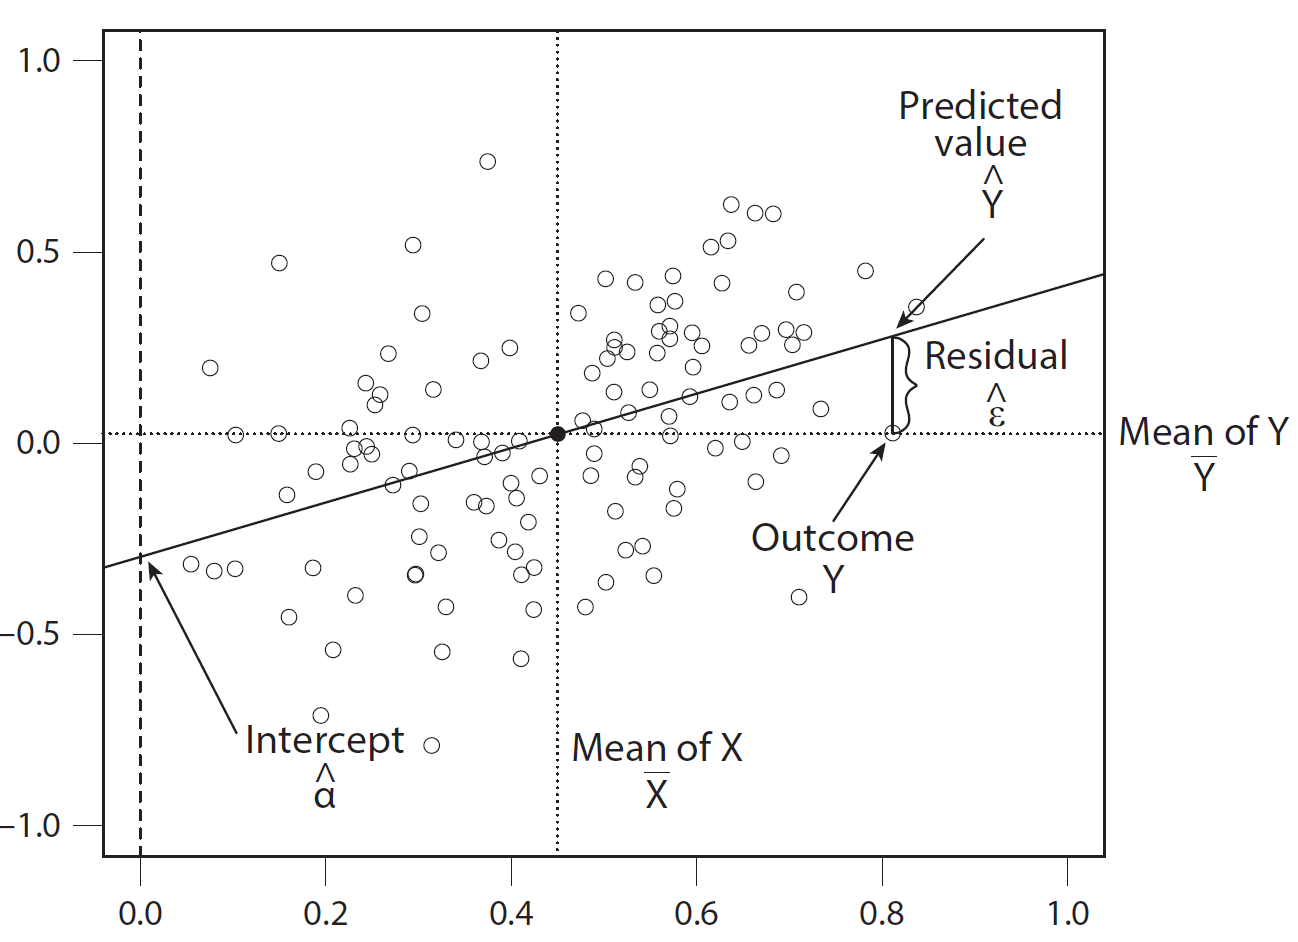
\includegraphics[scale=0.3]{img/RLM.png}
\end{center}
\end{frame}

\begin{frame}{Interpretation of the OLS estimators, fitted values, and residuals}

\begin{itemize}
    \item \textbf{The OLS estimators are estimators} of the unknown population parameters $\beta_0, \ldots, \beta_k$
    \vspace{0.3cm}

    \item \textbf{The fitted values are estimators} of the mean of the response given the predictor, that is, $\Esp[Y | X]$
    \vspace{0.3cm}

    \item \textbf{The residuals are estimators} of the error term
\end{itemize}

\end{frame}

\section{\Large Measures of fit}

\begin{frame}{Measures of fit in the MLR}

Three commonly used summary statistics in multiple regression are
\vspace{0.2cm}

\begin{itemize}
    \item the \textbf{Standard Error of the Regression} ($\SER$)
    \item the \textbf{coefficient of determination of the regression} $(\Rcoef)$
    \item the \textbf{adjusted $\pmb{\Rcoef}$} ($\adjRcoef$)
\end{itemize} 
\vspace{0.3cm}

All three statistics measure how well the OLS estimate of the multiple regression line describes, or ``fits'', the data.

\end{frame}

%--

\begin{frame}{The Standard Error of the Regression}

The standard error of the regression ($\SER$) \textbf{estimates the standard deviation of the error term} $u_i$
\vspace{0.3cm}

The $\SER$ \textbf{is a measure of the spread of the distribution of $Y$ around the regression line} 
\vspace{0.3cm}

In multiple regression, the $\SER$ is defined as
$$
\SER = \sqrt{\frac{\SSR}{n-k-1}}, 
$$
where $k$ is the number of predictors in the regression and $\SSR$ is the Sum of Squared Residuals, that is,
$$
\SSR = \sum_{i=1}^n \what{u}_i^2.
$$
\end{frame}

%--

\begin{frame}{The $\Rcoef$}

The regression \textbf{$\pmb{\Rcoef}$ is the fraction of the sample variance of $\pmb{Y_i}$ explained by (or predicted by) the regressors:} 
$$
\Rcoef = \frac{\ESS}{\TSS},
$$
where $\ESS$ is the Explained Sum of Squares and $\TSS$ is the Total Sum of Squares, that is,
$$
\ESS = \sum_{i=1}^n (\what{Y}_i - \oline{Y})^2,\quad \TSS = \sum_{i=1}^n (Y_i - \oline{Y})^2.
$$
\vspace{0.1cm}

Equivalently, since $\TSS = \SSR + \ESS$, the $\Rcoef$ is $1$ minus the fraction of the variance of $Y_i$ not explained by the regressors: 
$$
\Rcoef = 1 - \frac{\SSR}{\TSS}.
$$

\end{frame}

%--

\begin{frame}{The misguidance of the $\Rcoef$. The adjusted $\Rcoef$}

\textbf{The $\Rcoef$ increases whenever a regressor is added}, unless the estimated coefficient on the added regressor is exactly $0$, which is practically impossible (probability $0$). 
\vspace{0.2cm}

The increase in the $\Rcoef$ after adding a new variable does not mean an actual improvement in the fit of the model. .
\vspace{0.2cm}

In this sense, \textbf{the $\pmb{\Rcoef}$ gives an inflated estimate of how well the regression fits the data in the MLR model}. 
\vspace{0.2cm}

To correct this effect, the corrected $\Rcoef$, or \textbf{$\pmb{\adjRcoef}$, is defined by deflating or reducing the $\pmb{\Rcoef}$ by some factor:}
$$
\adjRcoef = 1 - \frac{n-1}{n-k-1}\frac{\SSR}{\TSS} = 1 - \frac{n-1}{n-k-1}(1 - \Rcoef),
$$
where $n$ is the sample size and $k$ is the number of regressors.
\vspace{0.3cm}

The $\adjRcoef$ does not necessarily increase when a new regressor is added.
\end{frame}

%--

% \begin{frame}{Model diagnosis}

%     \begin{center}
% \begin{tcolorbox}[enhanced,sharp corners,
%     width=8.2cm,
%     colback=white,
%     overlay={
%         % Upper left corner (quotation mark)
%         \node[anchor=north west,fill=white,draw=white,circle,inner sep=1pt] 
%         at ([xshift=-0.17cm,yshift=0.2cm]frame.north west) {\faQuoteLeft};
%         % Lower right corner (quotation mark)
%         \node[anchor=south east,fill=white,draw=white,circle,inner sep=1pt] 
%         at ([xshift=0.17cm,yshift=-0.2cm]frame.south east) {\faQuoteRight};
%     }
%     ]
%     % An object followed by another, and where [...], if the first object had not been, the second never had existed. \\
%     All models are wrong, but some are useful \\
%     \vspace{0cm}

%     {\small - George Box}
% \end{tcolorbox}
% \vspace{1cm}

% How to check the model assumptions?
% \end{center}
    
% \end{frame}

% \begin{frame}{Model diagnosis. Graphs}

% To check the model assumptions we will focus on \textbf{three diagnostic plots}:
% \vspace{0.1cm}

% \begin{enumerate}
    
%     \item \textbf{Residuals vs. fitted values plot.} This plot serves mainly to check the linearity, although lack of homoscedasticity or independence can also be detected.

%     \item \textbf{Q-Q plot.} Checks the normality of the error term.

%     \item \textbf{Scale-location plot.} Serves for checking the homoscedasticity. It is similar to the first diagnostic plot, but now with the residuals standardized and transformed by a square root (of the absolute value). This change transforms the task of spotting heteroskedasticity by looking into irregular vertical dispersion patterns into spotting for nonlinearities, which is somehow simpler.
    
% \end{enumerate}
    
% \end{frame}

% %--

% \begin{frame}{Model diagnosis. Residuals vs. fitted values plot}

% This plot serves mainly to check the linearity, although lack of homoscedasticity or independence can also be detected.
% \vspace{0.4cm}

% \begin{minipage}{0.5\textwidth}
%     \centering
%     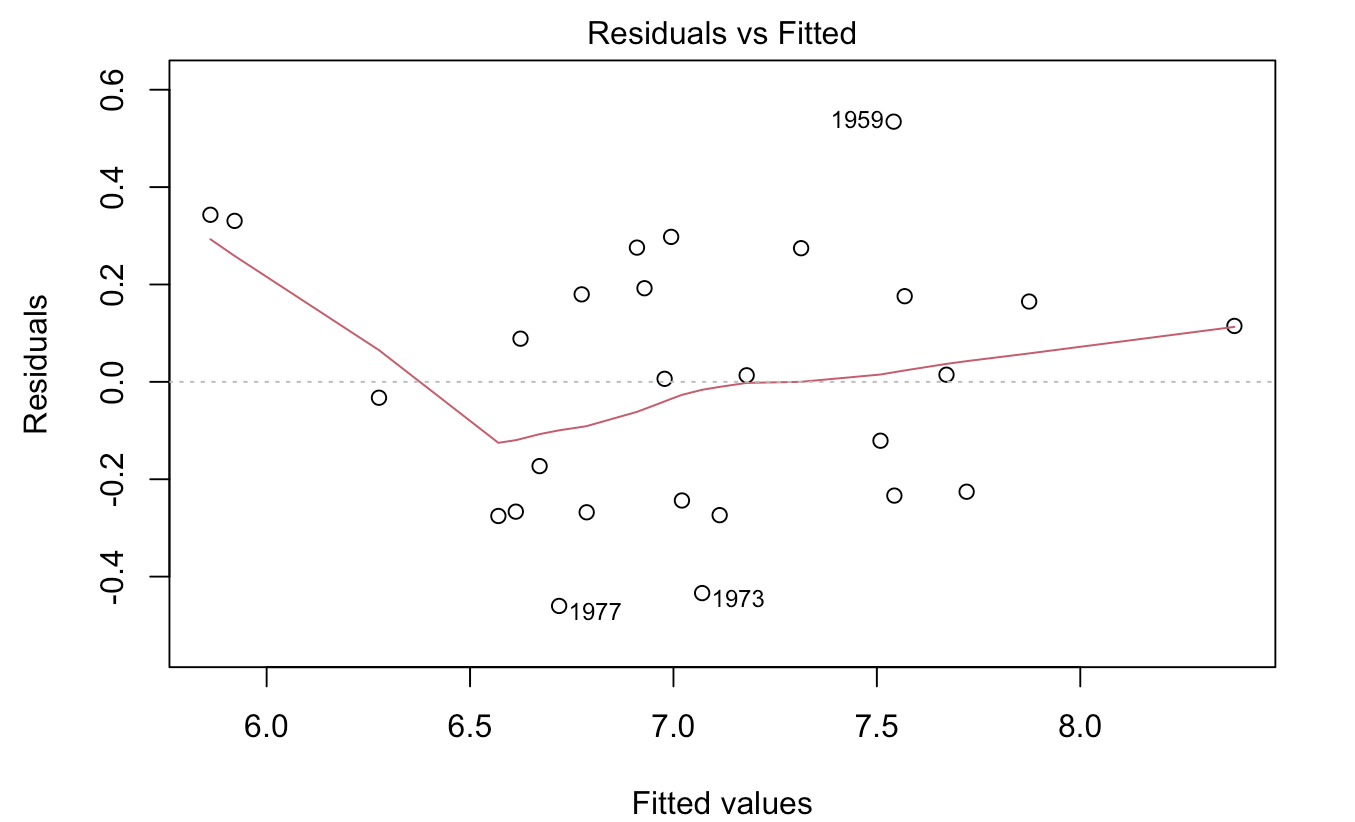
\includegraphics[scale = 0.4]{img/residuals-vs-fitted.png} 
% \end{minipage}
% \begin{minipage}{0.45\textwidth}
%     \textbf{Under linearity,} we expect the \textbf{red line} (a nonlinear fit of the mean of the residuals) \textbf{to be almost flat}.
%     \vspace{0.2cm}

%     \textbf{Heteroskedasticity can be detected} in the form of irregular vertical dispersion around the red line. 
%     \vspace{0.2cm}

%     \textbf{The dependence between residuals can be detected} (harder) in the form of non-randomly spread residuals.
% \end{minipage}
    
% \end{frame}

% %--

% \begin{frame}{Model diagnosis. Q-Q plot}

% \begin{minipage}{0.5\textwidth}
%     \centering
%     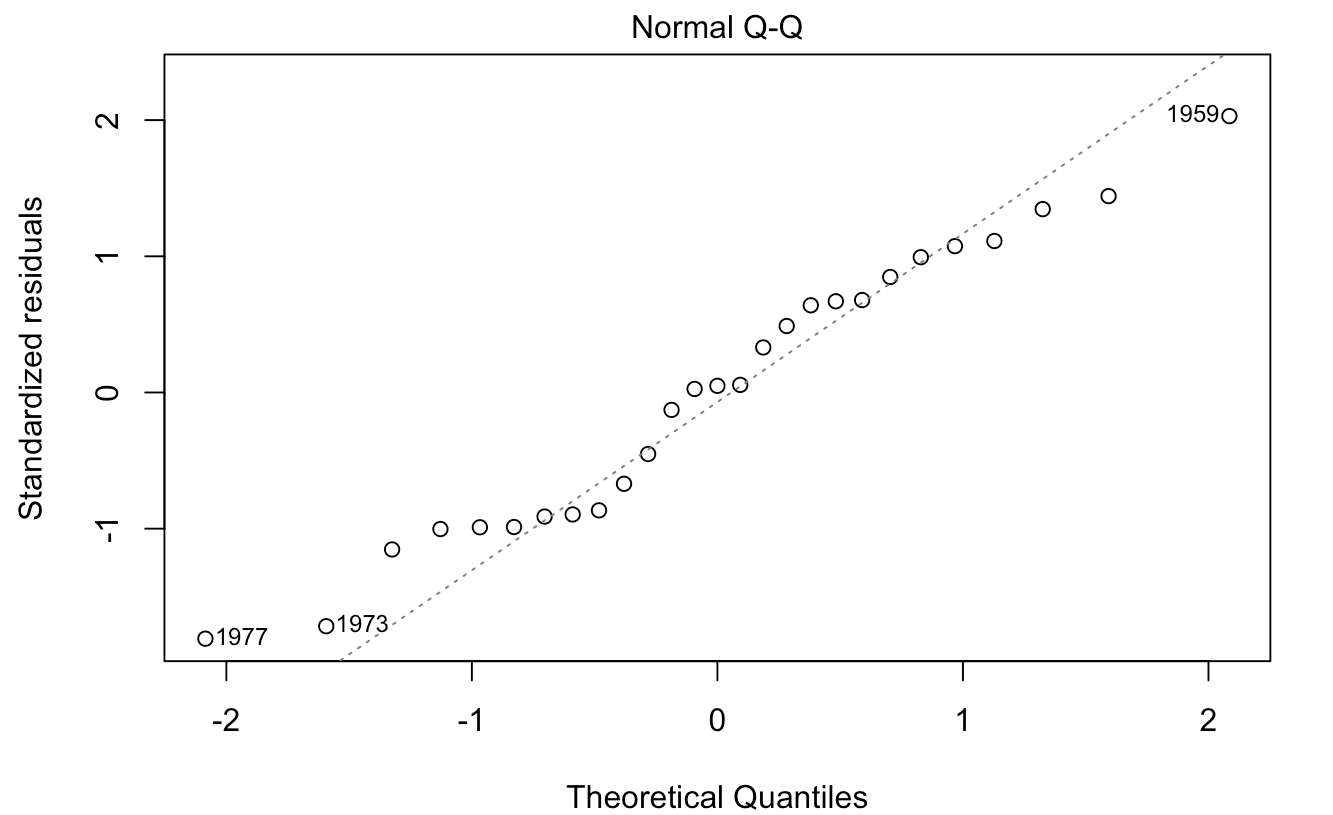
\includegraphics[scale = 0.4]{img/Q-Q-plot.png} 
% \end{minipage}
% \begin{minipage}{0.45\textwidth}
%     \textbf{Under normality, we expect the points} (sample quantiles of the standardized residuals vs. theoretical percentiles of a $\mathcal{N}(0, 1)$ \textbf{to align with the diagonal line}, which represents the ideal position of the points if those were sampled from a $\mathcal{N}(0, 1)$
%     \vspace{0.3cm}
    
%     \textbf{It is usual to have larger departures from the diagonal in the extremes} than in the center, even under normality, although these departures are more clear if the data is non-normal
% \end{minipage}
    
% \end{frame}

% %--

% \begin{frame}{Model diagnosis. Standardized residuals vs. fitted values plot}

% \begin{minipage}{0.5\textwidth}
%     \centering
%     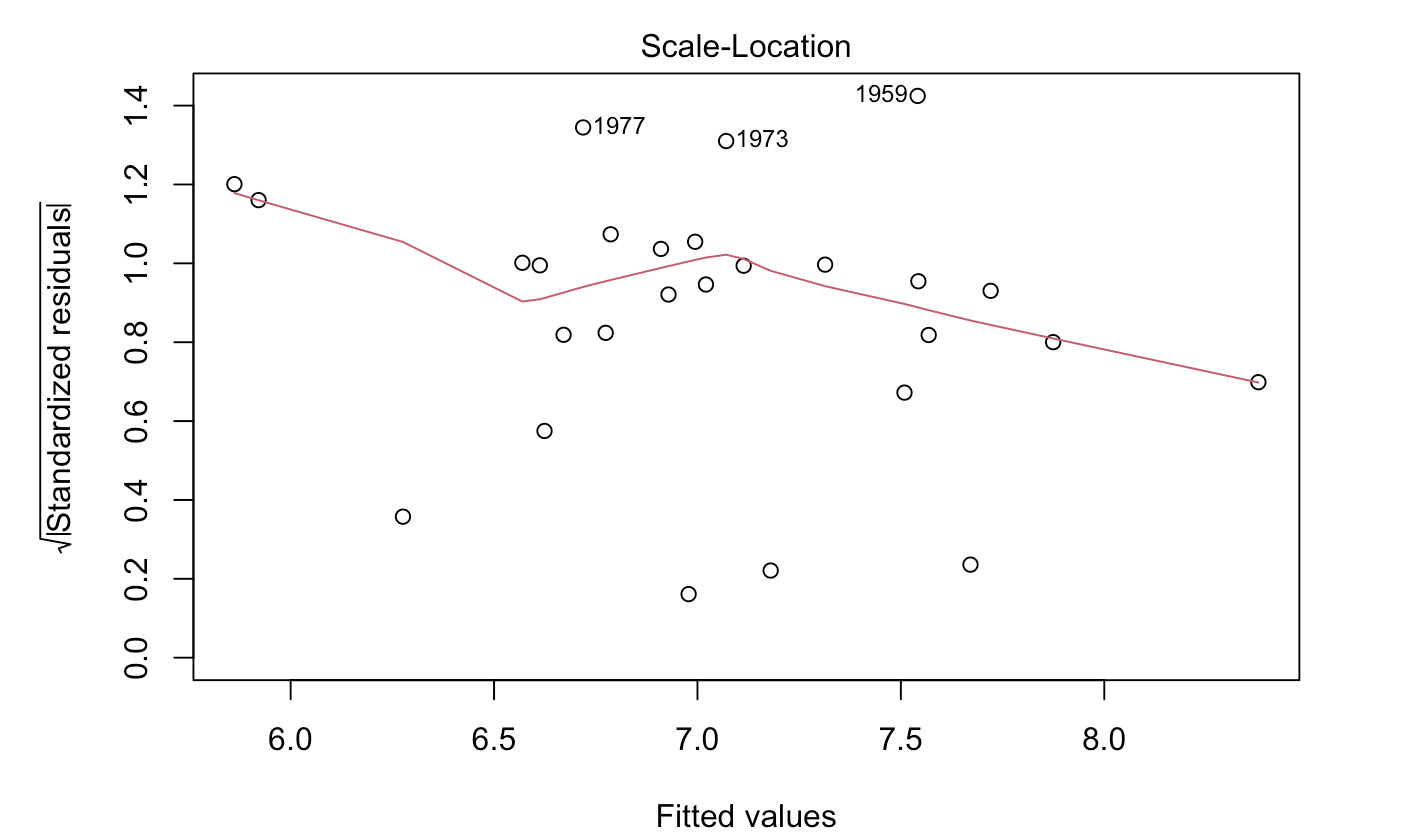
\includegraphics[scale = 0.4]{img/standard-residuals-vs-fitted.png} 
% \end{minipage}
% \begin{minipage}{0.45\textwidth}
%     \textbf{Serves for checking the homoscedasticity.} The residuals standardized and transformed by a square root (of the absolute value). 
%     \vspace{0.3cm}

%     \textbf{Heteroskedasticity can be detected by spotting nonlinearities.}
%     \vspace{0.3cm}
    
%     \textbf{Under homoscedasticity, we expect the red line to be almost flat.} If there are consistent nonlinear patterns, then there is evidence of heteroskedasticity.
% \end{minipage}
    
% \end{frame}

% %--

% \begin{frame}{Model diagnosis. Valid vs Problematic models}

% \vspace{-0.2cm}

% \centering
% {\tiny Examples of diagnostic plots of valid (left column) vs problematic models (right column)}
% \vspace{0.1cm}

% \begin{minipage}{0.32\textwidth}
%     \centering
%     {\tiny Residuals vs fitted values}
%     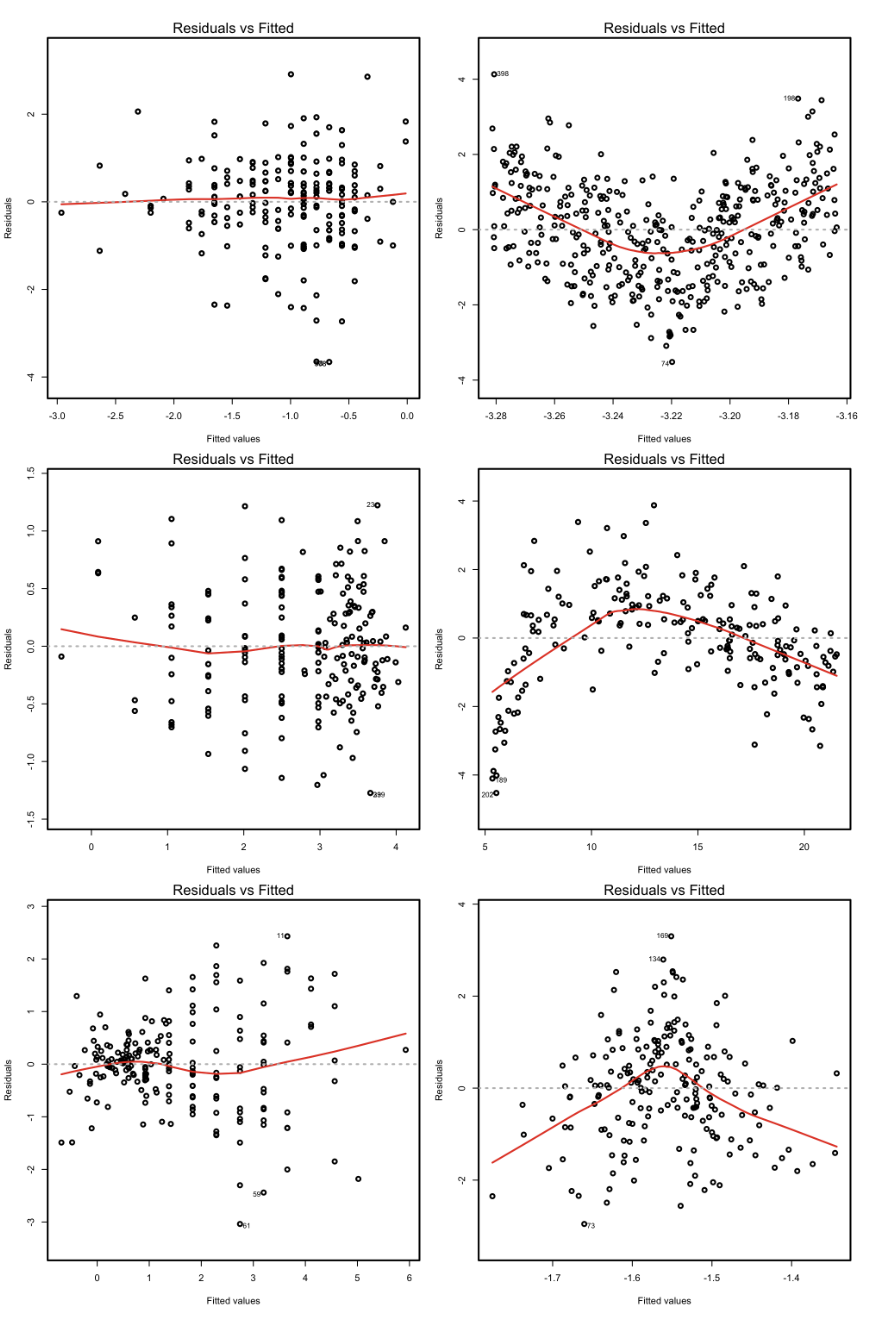
\includegraphics[scale = 0.4]{img/residual-vs-fitted-plots.png} 
% \end{minipage}
% \begin{minipage}{0.32\textwidth}
%     \centering
%     {\tiny Q-Q plot}
%     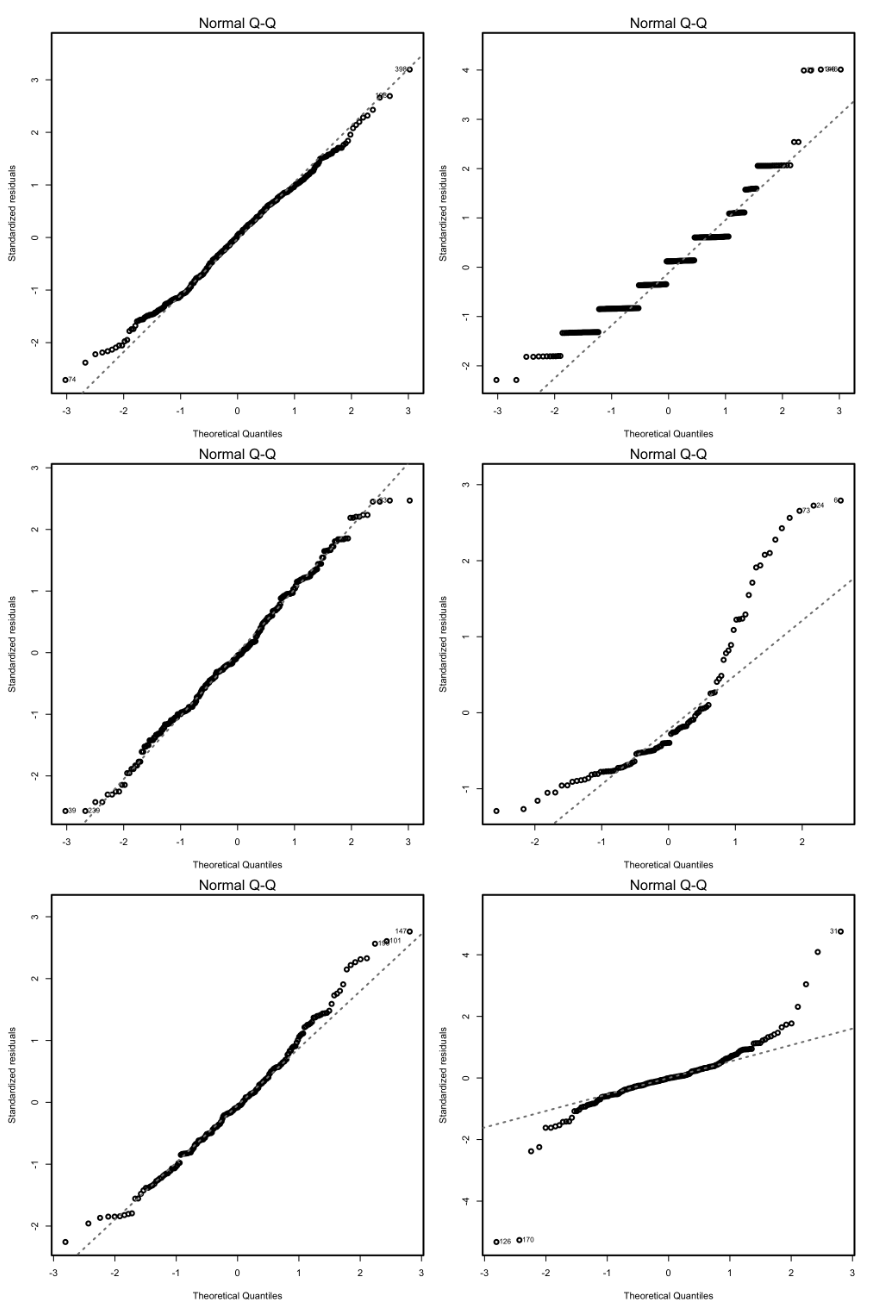
\includegraphics[scale = 0.4]{img/QQ-plots.png} 
% \end{minipage}
% \begin{minipage}{0.32\textwidth}
%     \centering
%     {\tiny Standard residuals vs fitted values}
%     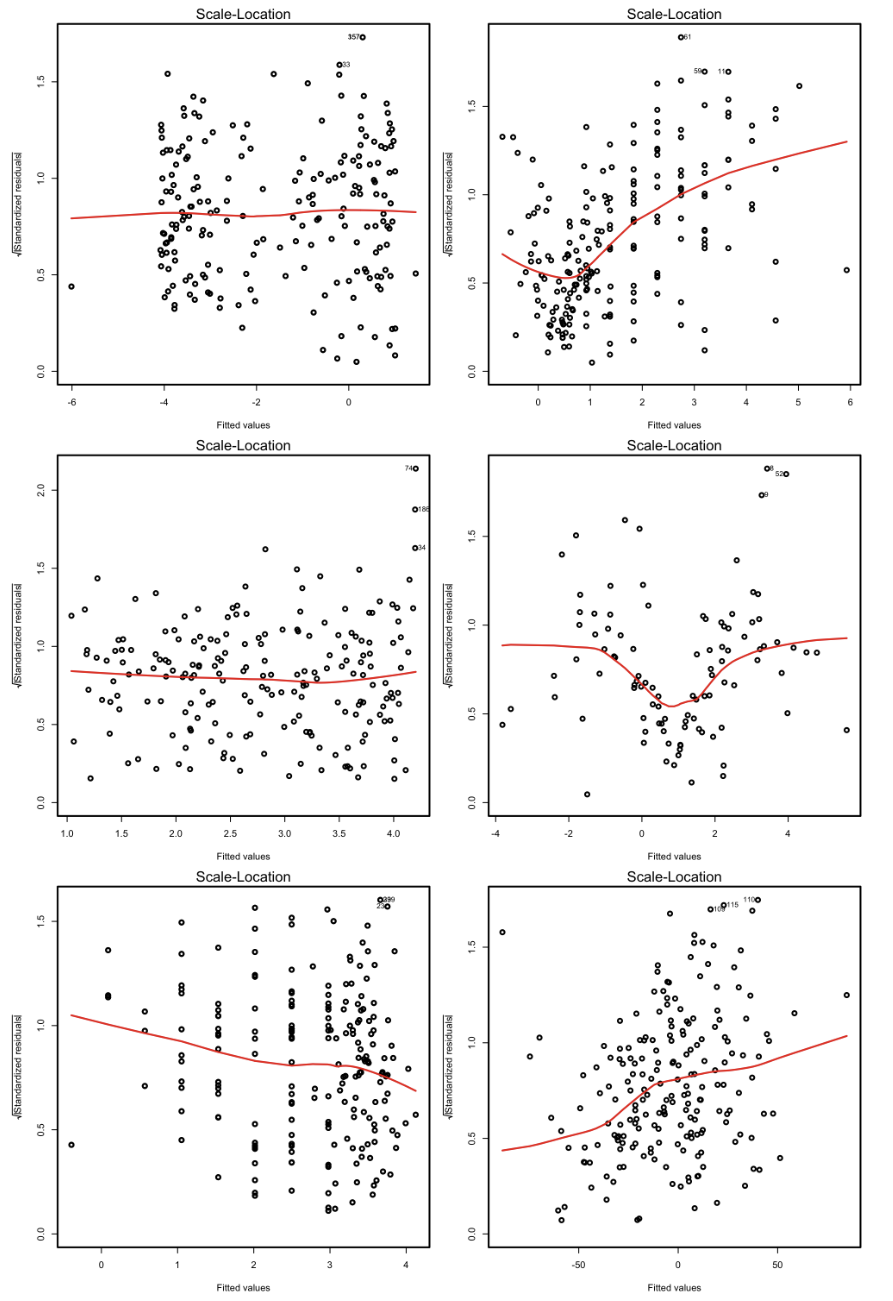
\includegraphics[scale = 0.4]{img/standard-residuals-vs-fitted-plots.png} 
% \end{minipage}
    
% \end{frame}

\section{\Large Prediction}

\begin{frame}{In-Sample Predictions in Linear Models}

\textbf{In-Sample Prediction:}  
\begin{itemize}
    \item Predictions made for the same data points used to fit the model.
    \item Also called fitted values.
    \item Assesses how well the model fits the training data.
    \item Evaluated using metrics like \( R^2 \), Mean Squared Error (MSE), or residuals.
    \item \textbf{Example:} Predicting house prices using the dataset used to train the model.
\end{itemize}

\end{frame}

\begin{frame}{Out-of-Sample Predictions in Linear Models}

\textbf{Out-of-Sample Prediction:}  
\begin{itemize}
    \item Predictions made for new, unseen data points not used during training.
    \item Measures the model's generalizability to other datasets.
    \item Typically evaluated using validation or test datasets.
    \item \textbf{Example:} Using a house price model trained on one dataset to predict prices in a different city.
\end{itemize}

\end{frame}

\begin{frame}{Within-Range Predictions in Linear Models}

\textbf{Within-Range Prediction:}  
\begin{itemize}
    \item Predictions made for data points within the range of predictor values observed during training.
    \item Outside range the model's assumptions may not hold.
    \item Provides reliable estimates since the model is not extrapolating.
    \item \textbf{Example:} Predicting house prices for properties with characteristics similar to (withing the range of) the training data.
\end{itemize}

% \textbf{Key Distinctions:}  
% \begin{itemize}
%     \item In-sample: Focuses on training data.  
%     \item Out-of-sample: Tests generalizability.  
%     \item Within-range: Ensures predictions stay within the model's domain of validity.
% \end{itemize}

\end{frame}

\begin{frame}{An example: facial appearance and election outcomes}

\vspace{-0.3cm}

\begin{center}
    \textbf{Does facial appearance predict election outcomes?}\footnote{\scriptsize Alexander Todorov, Anesu N. Mandisodza, Amir Goren, and Crystal C. Hall (2005) Inferences of competence from faces predict election outcomes.}    
    \vspace{0.4cm}
\end{center}

\begin{center}
\hspace{-1.3cm}
\begin{minipage}{0.3\textwidth}
    \begin{center}
        {\Large \href{url}{Case Study!}}
    \end{center}
\end{minipage}
\hspace{1cm}
\begin{minipage}{0.45\textwidth}
    \begin{center}
        
\includegraphics[width=7cm]{img/faces.png} % Adjust the width as needed
    
        \hspace{0.2cm} {\small Which person is the most competent?}    
    \end{center}
\end{minipage}
\end{center}
    
\end{frame}

\section{\Large Nonlinear models}

\begin{frame}{Nonlinear models}

The linear model is termed linear not because the regression curve is a line, but because \textbf{the effects of the parameters $\pmb{\beta_0}$ and $\pmb{\beta_1}$ are linear.} 
\vspace{0.4cm}

Indeed, \textbf{the predictor $\pmb{X}$ may exhibit a nonlinear effect on the response $\pmb{Y}$ and still be a linear model!} 
\vspace{0.4cm}

For example, the following models \textbf{can be transformed into simple linear models}, by considering the relation between $Y$ and the new regressor $\widetilde{X}$:
\vspace{0.2cm}

\begin{itemize}
    \item $Y = \beta_0 + \beta_1X^2 + u,\quad \widetilde{X} = X^2$
    \item $Y = \beta_0 + \beta_1\ln(X) + u,\quad \widetilde{X} = \ln(X)$
    \item $Y = \beta_0 + \beta_1(X^3 + \ln(|X|) + X^2) + u,\quad \widetilde{X} = X^3 + \ln(|X|) + X^2$
\end{itemize}

\end{frame}

%--

\begin{frame}{Nonlinear models}

This ``linearization trick'' is a simple way to \textbf{extend enormously the functionality of the linear model.} 
\vspace{0.4cm}

Indeed, the new transformed regression takes the form
$$
\pmb{Y = \beta_0 + \beta_1 f(X) + u,}
$$
where $f$ could be any function whose domain admits the values of the regressor.
\vspace{0.4cm}

This is \textbf{particularly useful in real applications}, where linearity is hardly verified.  
\vspace{0.4cm}

Some of \textbf{the most commonly used transformations} are:
\vspace{0.1cm}

\begin{itemize}
    \item (Polinomial) $f(x) = x^k,\ k\in \N$
    \item (Roots) $f(x) = x^{1/k},\ k\in \N$
    \item (Exponential) $f(x) = e^x,\ f(x) = e^{-x}$
    \item (Logarithmic) $f(x) = \ln(x)$
\end{itemize}

\end{frame}

%--

\begin{frame}{Nonlinear models}

\centering
Quadratic pattern $Y$ vs $X$ (left) and Linearized pattern $Y$ vs $X^2$ (right)
 
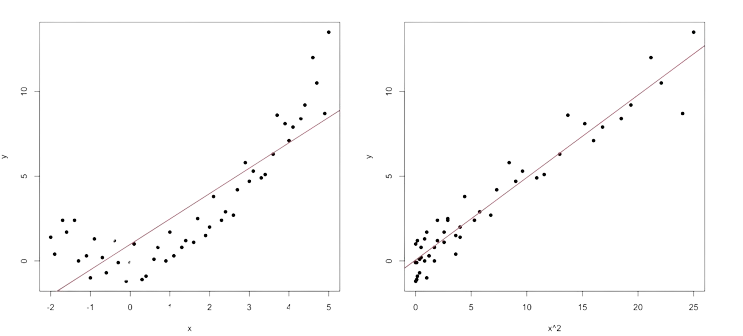
\includegraphics[scale=0.45]{img/linear-transformation.png}

You can visualize more transformations \href{https://shinyserv.es/shiny/non-linear/}{here}

\end{frame}

%--

\begin{frame}{Nonlinear models. General case}

\textbf{We can also transform the response} to achieve linearity,
\vspace{0.4cm}

In such a case, \textbf{the general transformed linear model} takes the form
$$
g(Y) = \beta_0 + \beta_1 f(X) + u,
$$
for two suitable functions $f$ and $g$.
\vspace{0.4cm}

\textbf{It is important for $\pmb{g}$ to be one-to-one}, to be able to explain the original variable $Y$ and not the transformation $g(Y)$.

\end{frame}

%--

% \section{\Large The linear model for causal inference}

% \begin{frame}{Linear regression and causation}
%     \begin{itemize}
%         \item Regression is most often used for making predictions.
%         \item How can regression be used to draw causal inference?
%         \item Recall that causal inference requires predicting/estimating the conterfactual ourcome
%         \item \textbf{Under certain assumptions}, regression models can be used to predict counterfactual outcomes.
%     \end{itemize}
% \end{frame}

% \begin{frame}{Conditional Independence in Linear Regression for Causal Inference}
%   \begin{itemize}
%     \item In the linear regression model
%       \[
%       Y = \alpha + \tau T + \beta X + u,
%       \]
%       the Conditional Independence Assumption (CIA) \( \mathbb{E}(u \mid T, X) = 0 \) ensures that the estimator \(\tau\) measures the causal effect of \(T\) on \(Y\).
%     % \item \textbf{Causal Inference:} With this assumption, any association captured by \(\tau\) can be interpreted causally, provided that all confounders are included in \(X\).
%     \item \textbf{Example:} Estimating the causal impact of exposure to political advertising on voter turnout.
%     \item \textbf{Variables:}
%       \begin{itemize}
%         \item \(T\): Exposure to political advertising (1 if exposed, 0 otherwise).
%         \item \(Y\): Voter turnout in a subsequent election.
%         \item \(X\): Baseline political engagement (e.g., previous voting history or political awareness).
%       \end{itemize}
%     \item \textbf{The CIA:} where controlling for baseline political engagement (\(X\)) supports the assumption \( \mathbb{E}(u \mid T, X) = 0 \).
%     \item \textbf{Interpretation:} Under the CIA, the coefficient \(\tau\) reflects the causal effect of political advertising exposure on increasing voter turnout.
%   \end{itemize}
% \end{frame}

% \section{\Large The linear model for causal inference}

% \begin{frame}{The assumptions of the model for causal inference}

% Some assumptions are required to ensure reliable and valid parameter estimates and inference, and for interpreting the results as causal effect . 
% \vspace{0.2cm}

% Assumptions for having unbiased OLS estimators representing causal relation:
% \begin{enumerate}    
%     \item[L1] \textbf{Linearity:} $Y = \beta X + u$

%     \item[L2] \textbf{Zero conditional mean:} $\Esp[u \mid X] = 0$ \\
%     The value of the regressors must contain no information about the mean of the unobserved factors
% \end{enumerate}
% \vspace{0.2cm}

% Other assumptions must be added for efficiency and inference of the OLS estimators:
% \begin{enumerate}
%     \item[L3] \textbf{Homoskedasticity:} $\operatorname{Var}(u \mid X) = \sigma^2$ \\
%     The variance of $u$ is constant across all values of $X$
    
%     \item[L4] \textbf{Normality:} $u \sim \mathcal{N}(0, \sigma^2)$
% \end{enumerate}

% \vspace{0.3cm}

% \end{frame}

\section{\Large The linear model for causal inference \\ under randomized control trials}

\begin{frame}{RCTs and Linear Regression Causal Inference: the binary (dummy) regressors case}

    \begin{itemize}
        \item For the sake of simplicity, let us consider a simple setting to illustrate the concept:
        $$
        Y = \beta_0 + \beta_1 X + u.
        $$
        \item $Y$ is the response
        \item $X$ is the binary treatment ($X = 1$ for treatment and $X = 0$ for control)
        \item When \(X\) is binary,
        \begin{align*}
            \what{\beta_0} &= \underbrace{\frac{1}{n_0} \sum_{i=1}^n (1-X_i) Y_i}_{\text{mean outcome for control}} \\
            \what{\beta_1} &= \underbrace{\frac{1}{n_1} \sum_{i=1}^n X_i Y_i}_{\text{mean outcome for treated}} - \underbrace{\frac{1}{n_0} \sum_{i=1}^n (1-X_i) Y_i}_{\text{mean outcome for control}}.    
        \end{align*}
    \item Therefore, \(\what{\beta_1}\) is the \textbf{difference-in-mean estimator} of the \textbf{estimated average treatment effect (ATE)}.
    \end{itemize}
\end{frame}

\begin{frame}{Linear regression as a difference-in-means estimator}

\begin{coolblock}{Linear regressions equivalence to difference-in-means estimators}
    When applied to \textbf{experimental data} with a single, \textbf{binary treatment}, \textbf{the estimated slope coefficient of the linear regression model can be interpreted as an estimate of average treatment effect and is numerically equivalent to the difference-in-means estimator}. 
    \vspace{0.2cm}
    
    The estimated intercept, on the other hand, is equal to the estimated average outcome under the control condition. The randomization of treatment assignment permits this causal interpretation of  association identified under a linear regression model.
\end{coolblock}
    
\end{frame}

\begin{frame}{Case Study. Simple regression}

    \begin{center}
        Do female politicians promote different policies than male politicians?\footnote{\scriptsize Raghabendra Chattopadhyay and Esther Duflo (2004) Women as policy makers: Evidence from a randomized policy experiment in India.}
        \vspace{1cm}

        {\Large \href{url}{Case Study!}}
    \end{center}
    
\end{frame}

\begin{frame}{Heterogeneous treatment effect}
    \begin{itemize}
        \item \textbf{Heterogeneous treatment effect} refers to the variation in the impact of a treatment across different individuals or groups (e.g., effect of drug between patients in different age ranges). 
        \item \textbf{The Simpson paradox:} when a trend observed in multiple groups changes when the groups are aggregated.
        \item \textbf{Linear regression with multiple predictors} can help uncover these variations by identifying characteristics associated with differences in the treatment effect's direction and magnitude.
        \item \textbf{Understanding} heterogeneous treatment effects is crucial for tailoring treatments to those who will benefit most and avoiding adverse outcomes for others. 
    \end{itemize}
\end{frame}

\begin{frame}{The Simpson Paradox}

    \begin{center}
        \animategraphics[loop, autoplay, width=0.6\linewidth]{12}{simpson/Simpsons_paradox_-_animation-}{0}{48}
        \vspace{0.3cm}

        \href{https://en.wikipedia.org/wiki/Simpson's_paradox}{Simpson Paradox!}
    \end{center}
    
\end{frame}

\begin{frame}{Introduction to Linear Regression with Interaction Terms}
    
    \textbf{Goal:} Model how the effect of a predictor (treatment) varies based on another (covariate) variable.
    
    \vspace{1em}
    \textbf{Example of linear regression with interaction:}
    \[
    Y = \beta_0 + \beta_1 X + \beta_2 Z + \beta_3 (X \cdot Z) + u
    \]

    \begin{itemize}
        \item \( X \): Treatment variable
        \item \( Z \): Covariate variable (e.g., age, gender, income)
        \item \( X \cdot Z \): \textbf{Interaction term} capturing the interaction effect
        \item \( \beta_3 \): Coefficient of interaction term, indicating how the effect of \( X \) changes with \( Z \)
    \end{itemize}
    
\end{frame}

\begin{frame}{Interaction coefficient interpretation. An example}

    \textbf{Example of linear regression with interaction:}
    \begin{align}\label{eq:linear_interaction}
        Y = \beta_0 + \beta_1 X + \beta_2 Z + \beta_3 (X \cdot Z) + u    
    \end{align}

    \begin{coolblock}{Interpretation of the interaction term}
        The linear model \eqref{eq:linear_interaction} with the interaction term $\beta_3(X \cdot Z)$ assumes that the effect of $X$ linearly depends on $Z$. That is, as we increase $Z$ by one unit, the change in the average outcome associated with a one-unit increase of $X$ goes up by $\beta_3$.
    \end{coolblock}
    \vspace{0.3cm}

    \begin{center}
        Interaction terms may also be non-linear, like $(X \cdot Z^2)$ or $(X \cdot \ln(Z))$.    
    \end{center}
    
\end{frame}

\begin{frame}{Case Study. Heterogeneous treatment effect. Categorical variables}

    \begin{center}
        Do social pressure increases participation in elections?\footnote{\scriptsize Alan S. Gerber, Donald P. Green, and Christopher W. Larimer (2008) Social pressure and voter turnout: Evidence from a large-scale field experiment.}
        \vspace{1cm}

        {\Large \href{url}{Case Study!}}
    \end{center}
    
\end{frame}

\section{\Large The linear model for causal inference \\ under observational studies}

\begin{frame}{Regression discontinuity design. Definition.}

\begin{coolblock}{Regression Discontinuity Design (RDD)}
    Quasi-experimental method used to estimate causal effects when a treatment is assigned based on a cutoff or threshold in a continuous variable.
\end{coolblock}

\begin{itemize}
    \item \textbf{Key Assumption:} Units just above and below the cutoff are similar in all respects except for the treatment received.
    \item \textbf{Assignation mechanism:} Observational units are assigned a score (e.g., income, age, or test scores), and treatment is assigned when this score crosses a predetermined threshold.
    \item \textbf{Applications:} Common in policy evaluation, such as the impact of scholarships awarded based on test scores or voting outcomes based on a minimum percentage.
    \item \textbf{Validity} Often has strong internal validity, but it may lack external validity because the result may not be generalizable to observations away from the point of discontinuity.
\end{itemize}
    
\end{frame}

\begin{frame}{Regression discontinuity design. Two regressions}
    
    \textbf{Regressions:}
    \begin{align*}
        Y_i &= \beta_0^{\text{control}} + \beta_1^{\text{control}} X_i + u_i, && \text{ for } i \text{ such that } X_i < c, \\
        Y_i &= \beta_0^{\text{treat}} + \beta_1^{\text{treat}} X_i + u_i, && \text{ for } i \text{ such that } X_i \geq c.
    \end{align*}
    
    \begin{itemize}
        \item \( Y \): Outcome variable.
        \item \( X \): Regressor, determines treatment assignment.
        \item \( c \): Cutoff threshold.
    \end{itemize}
    \vspace{0.3cm}
    
    \textbf{ATE estimation:}
    \begin{align*}
        \lim_{X \to c^+} E[Y|X] - \lim_{X \to c^-} E[Y|X] 
        &= (\beta_0^{\text{treat}} + \beta_1^{\text{treat}} c) - (\beta_0^{\text{control}} + \beta_1^{\text{control}} c) \\
        &= (\beta_0^{\text{treat}} - \beta_0^{\text{control}}) + c(\beta_1^{\text{treat}} - \beta_1^{\text{control}})
    \end{align*}

\end{frame}

\begin{frame}{Regression discontinuity design. One regression}
    \textbf{Regression:}
    $
    Y = \beta_0 + \beta_1 X + \beta_2 T + \beta_3 T \cdot X + u
    $
    \begin{itemize}
        \item \( Y \): Outcome variable.
        \item \( X \): Regressor, determines treatment assignment.
        \item \( T \): Treatment indicator \( (T = 1 \text{ if } X \geq c, 0 \text{ otherwise}) \).
        \item \( c \): Cutoff threshold.
    \end{itemize}
    \vspace{0.3cm}
    
    \textbf{ATE estimation:}
    \begin{align*}
        \lim_{X \to c^+} E[Y|X] - \lim_{X \to c^-} E[Y|X] 
        &= (\beta_0 + \beta_1 c) - (\beta_0 + \beta_1 c) 
        = \beta_2 + \beta_3 c
    \end{align*}
    
    \textbf{Connection with the two-regressions case}
    $$
    \beta_0 = \beta_0^\text{control}, \quad \beta_1 = \beta_1^{\text{control}}, \quad \beta_0 + \beta_2 = \beta_0^\text{treat}, \quad \beta_1 + \beta_3 = \beta_1^{\text{treat}}
    $$
\end{frame}

\begin{frame}{Regression discontinuity design. Visualization}

\begin{minipage}{0.29\textwidth}
   { \hspace{0.2cm} \textbf{Example:} scholarships are awarded to students scoring above 80 on a test. Plot average test scores on the x-axis and the likelihood of college enrollment on the y-axis, showing a clear jump at the cutoff.}
\end{minipage}
\hspace{0.5cm}
\begin{minipage}{0.65\textwidth}
    \begin{center}
    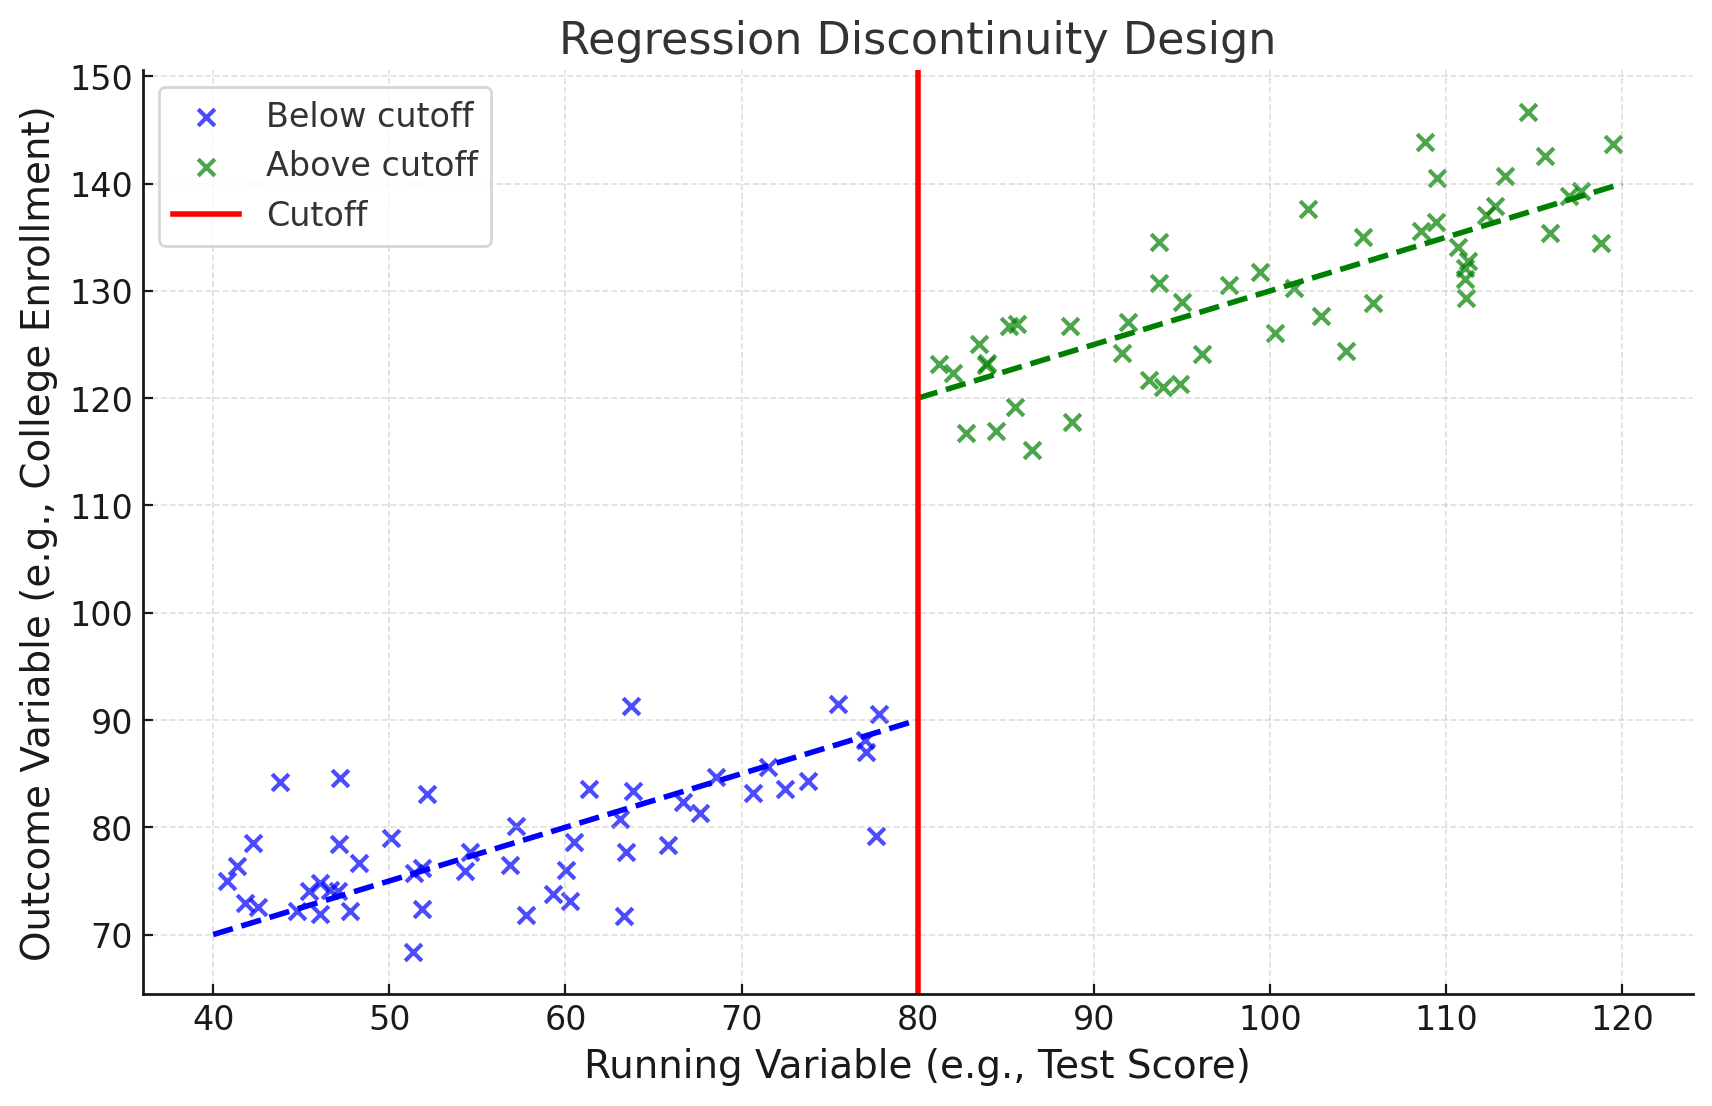
\includegraphics[scale=0.41]{img/RDD.png}
\end{center}    
\end{minipage}
    
\end{frame}

\begin{frame}{Case Study. RDD}

    \begin{center}
        Can politicians increase their personal wealth due to holding office?\footnote{\scriptsize Andrew C. Eggers and Jens Hainmueller (2009) MPs for sale? Returns to office in postwar British politics.}
        \vspace{1cm}

        {\Large \href{url}{Case Study!}}
    \end{center}
    
    
\end{frame}

\end{document}
